%%% The main file. It contains definitions of basic parameters and includes all other parts.

%% Settings for single-side (simplex) printing
% Margins: left 40mm, right 25mm, top and bottom 25mm
% (but beware, LaTeX adds 1in implicitly)
\documentclass[12pt,a4paper]{report}
\setlength\textwidth{145mm}
\setlength\textheight{247mm}
\setlength\oddsidemargin{15mm}
\setlength\evensidemargin{15mm}
\setlength\topmargin{0mm}
\setlength\headsep{0mm}
\setlength\headheight{0mm}
% \openright makes the following text appear on a right-hand page
\let\openright=\clearpage

%% Settings for two-sided (duplex) printing
% \documentclass[12pt,a4paper,twoside,openright]{report}
% \setlength\textwidth{145mm}
% \setlength\textheight{247mm}
% \setlength\oddsidemargin{14.2mm}
% \setlength\evensidemargin{0mm}
% \setlength\topmargin{0mm}
% \setlength\headsep{0mm}
% \setlength\headheight{0mm}
% \let\openright=\cleardoublepage

%% Generate PDF/A-2u
\usepackage[a-2u]{pdfx}

%% Character encoding: usually latin2, cp1250 or utf8:
\usepackage[utf8]{inputenc}

%% Prefer Latin Modern fonts
\usepackage{lmodern}

%% Further useful packages (included in most LaTeX distributions)
\usepackage{amsmath}        % extensions for typesetting of math
\usepackage{amsfonts}       % math fonts
\usepackage{amsthm}         % theorems, definitions, etc.
\usepackage{bbding}         % various symbols (squares, asterisks, scissors, ...)
\usepackage{bm}             % boldface symbols (\bm)
\usepackage{graphicx}       % embedding of pictures
\usepackage{fancyvrb}       % improved verbatim environment
\usepackage{natbib}         % citation style AUTHOR (YEAR), or AUTHOR [NUMBER]
\usepackage[nottoc]{tocbibind} % makes sure that bibliography and the lists
			    % of figures/tables are included in the table
			    % of contents
\usepackage{dcolumn}        % improved alignment of table columns
\usepackage{booktabs}       % improved horizontal lines in tables
\usepackage{paralist}       % improved enumerate and itemize
\usepackage[usenames]{xcolor}  % typesetting in color

%%% Basic information on the thesis

% Thesis title in English (exactly as in the formal assignment)
\def\ThesisTitle{Planning for Transportation Problems}

% Author of the thesis
\def\ThesisAuthor{Ondrej Škopek}

% Year when the thesis is submitted
\def\YearSubmitted{2017}

% Name of the department or institute, where the work was officially assigned
% (according to the Organizational Structure of MFF UK in English,
% or a full name of a department outside MFF)
\def\Department{Department of Theoretical Computer Science and Mathematical Logic}

% Is it a department (katedra), or an institute (ústav)?
\def\DeptType{Department}

% Thesis supervisor: name, surname and titles
\def\Supervisor{prof. RNDr. Roman Barták, Ph.D.}

% Supervisor's department (again according to Organizational structure of MFF)
\def\SupervisorsDepartment{Department of Theoretical Computer Science and Mathematical Logic}

% Study programme and specialization
\def\StudyProgramme{Computer Science}
\def\StudyBranch{General Computer Science}

% An optional dedication: you can thank whomever you wish (your supervisor,
% consultant, a person who lent the software, etc.)
\def\Dedication{%
Dedication.
}

% Abstract (recommended length around 80-200 words; this is not a copy of your thesis assignment!)
\def\Abstract{%
Abstract.
}

% 3 to 5 keywords (recommended), each enclosed in curly braces
\def\Keywords{%
{planning}, {transport}, {logistics}
}% TODO: Should have commas?

%% The hyperref package for clickable links in PDF and also for storing
%% metadata to PDF (including the table of contents).
%% Most settings are pre-set by the pdfx package.
\hypersetup{unicode}
\hypersetup{breaklinks=true}

% Definitions of macros (see description inside)
%%% This file contains definitions of various useful macros and environments %%%
%%% Please add more macros here instead of cluttering other files with them. %%%

%%% Minor tweaks of style

% These macros employ a little dirty trick to convince LaTeX to typeset
% chapter headings sanely, without lots of empty space above them.
% Feel free to ignore.
\makeatletter
\def\@makechapterhead#1{
  {\parindent \z@ \raggedright \normalfont
   \Huge\bfseries \thechapter. #1
   \par\nobreak
   \vskip 20\p@
}}
\def\@makeschapterhead#1{
  {\parindent \z@ \raggedright \normalfont
   \Huge\bfseries #1
   \par\nobreak
   \vskip 20\p@
}}
\makeatother

% This macro defines a chapter, which is not numbered, but is included
% in the table of contents.
\def\chapwithtoc#1{
\chapter*{#1}
\addcontentsline{toc}{chapter}{#1}
}

% Draw black "slugs" whenever a line overflows, so that we can spot it easily.
\overfullrule=1mm

%%% Macros for definitions, theorems, claims, examples, ... (requires amsthm package)

\theoremstyle{plain}
\newtheorem{thm}{Theorem}
\newtheorem{lemma}[thm]{Lemma}
\newtheorem{claim}[thm]{Claim}

\theoremstyle{plain}
\newtheorem{defn}{Definition}

\theoremstyle{remark}
\newtheorem*{cor}{Corollary}
\newtheorem*{rem}{Remark}
\newtheorem*{example}{Example}

%%% An environment for proofs

%%% FIXME %%% \newenvironment{proof}{
%%% FIXME %%%   \par\medskip\noindent
%%% FIXME %%%   \textit{Proof}.
%%% FIXME %%% }{
%%% FIXME %%% \newline
%%% FIXME %%% \rightline{$\square$}  % or \SquareCastShadowBottomRight from bbding package
%%% FIXME %%% }

%%% An environment for typesetting of program code and input/output
%%% of programs. (Requires the fancyvrb package -- fancy verbatim.)

\DefineVerbatimEnvironment{code}{Verbatim}{fontsize=\small, frame=single}

%%% The field of all real and natural numbers
\newcommand{\R}{\mathbb{R}}
\newcommand{\N}{\mathbb{N}}

%%% Useful operators for statistics and probability
\DeclareMathOperator{\pr}{\textsf{P}}
\DeclareMathOperator{\E}{\textsf{E}\,}
\DeclareMathOperator{\var}{\textrm{var}}
\DeclareMathOperator{\sd}{\textrm{sd}}

%%% Transposition of a vector/matrix
\newcommand{\T}[1]{#1^\top}

%%% Various math goodies
\newcommand{\goto}{\rightarrow}
\newcommand{\gotop}{\stackrel{P}{\longrightarrow}}
\newcommand{\maon}[1]{o(n^{#1})}
\newcommand{\abs}[1]{\left|{#1}\right|}
\newcommand{\dint}{\int_0^\tau\!\!\int_0^\tau}
\newcommand{\isqr}[1]{\frac{1}{\sqrt{#1}}}

%%% Various table goodies
\newcommand{\pulrad}[1]{\raisebox{1.5ex}[0pt]{#1}}
\newcommand{\mc}[1]{\multicolumn{1}{c}{#1}}

%% Personal:
\newcommand{\TODO}[1]{\textbf{TODO} [{\color{red}#1}]}
\newcommand{\comment}[1]{}

\DeclareMathOperator{\noop}{\textrm{no-op}}

% Title page and various mandatory informational pages
\begin{document}
%%% Title page of the thesis and other mandatory pages

%%% Title page of the thesis

\pagestyle{empty}
\hypersetup{pageanchor=false}
\begin{center}

\centerline{\mbox{\includegraphics[width=166mm]{../img/logo-en.pdf}}}

\vspace{-8mm}
\vfill

{\bf\Large BACHELOR THESIS}

\vfill

{\LARGE\ThesisAuthor}

\vspace{15mm}

{\LARGE\bfseries\ThesisTitle}

\vfill

\Department

\vfill

\begin{tabular}{rl}

Supervisor of the bachelor thesis: & \Supervisor \\
\noalign{\vspace{2mm}}
Study programme: & \StudyProgramme \\
\noalign{\vspace{2mm}}
Study branch: & \StudyBranch \\
\end{tabular}

\vfill

% Zde doplňte rok
Prague \YearSubmitted

\end{center}

\newpage

%%% Here should be a bound sheet included -- a signed copy of the "bachelor
%%% thesis assignment". This assignment is NOT a part of the electronic
%%% version of the thesis. DO NOT SCAN.

%%% A page with a solemn declaration to the bachelor thesis

\openright
\hypersetup{pageanchor=true}
\pagestyle{plain}
\pagenumbering{roman}
\vglue 0pt plus 1fill

\noindent
I declare that I carried out this bachelor thesis independently, and only with the cited
sources, literature and other professional sources.

\medskip\noindent
I understand that my work relates to the rights and obligations under the Act No.~121/2000 Sb.,
the Copyright Act, as amended, in particular the fact that the Charles
University has the right to conclude a license agreement on the use of this
work as a school work pursuant to Section 60 subsection 1 of the Copyright Act.

\vspace{10mm}

\hbox{\hbox to 0.5\hsize{%
In Prague,  \ThesisDate
\hss}\hbox to 0.5\hsize{%
\ThesisAuthor
\hss}}

\vspace{20mm}
\newpage

%%% Mandatory information page of the thesis

\openright

\vbox to 0.5\vsize{
\setlength\parindent{0mm}
\setlength\parskip{5mm}

Title:
\ThesisTitle

Author:
\ThesisAuthor

\DeptType:
\Department

Supervisor:
\Supervisor, \SupervisorsDepartment

Abstract:
\Abstract

Keywords:
\Keywords

\vss}

\newpage

%%% Dedication

\openright

\noindent
\Dedication

\newpage

\openright
\pagestyle{plain}
\pagenumbering{arabic}
\setcounter{page}{1}


%%% A page with automatically generated table of contents of the bachelor thesis

\tableofcontents

%%% Each chapter is kept in a separate file
\chapter*{Introduction}
\addcontentsline{toc}{chapter}{Introduction}


\chapter{Analysis of transportation planning problems}

In this chapter, we formalize the concept of planning to help us with formally introducing the studied transportation problems. We will also briefly discuss specifics of the Transport domain and mention similar studied problems.

\section{Context}

\TODO{Title + VRP, \citep{Dantzig1959}}


\subsection{The Vehicle Routing Problem}

\TODO{mention Dantzig} \citep{Dantzig1959}

\TODO{mention Braekers} \citep{Braekers2016}

\TODO{mention Montoya} \citep{Montoya-Torres2015}

\TODO{mention Neo} \citep{ResearchGroup2013}

\subsubsection{Constraint Satisfaction Problems}

\subsubsection{Problem formulation}

\subsubsection{Comparison to the Transport domain formulation}

\subsubsection{Formulating the sequential Transport domain as a VRP problem}

\TODO{Ghallab 8.3}

\subsection{Past solutions and approaches}

\TODO{\ldots see \citep{Skopek2017}}

\section{Automated planning}

Planning is usually defined as the reasoning side of acting -- an abstract deliberation
process that chooses and organizes actions by anticipating their outcomes. \citep[Section~1.1]{Ghallab2004}
It seems only natural that we want to have computers to do this strenuous activity for us.
Automated planning is an attempt at just that -- it is an area of Artificial Intelligence (AI) that
studies the planning process computationally. \citep[Section~1.1]{Ghallab2004}

Unfortunately, the specific situations in which we want to use automated planning are very diverse --
from devising a sequence of actions to shut down a nuclear power plant to planning the robotic arm
movements in an assembly line or devising the complex motor activations for space aircraft positioning.
Due to this, people are often interested in domain-independent planning, where the planner gets information
about both the domain and the specific problem and attempts to devise a plan using only the provided knowledge
and the planner's previously built-in processes. \citep[Section~1.3]{Ghallab2004}

On the other hand, domain-specific planning, where domain knowledge has been built into the planner,
has obvious advantages when solving problems in that domain -- all the while being useless on problems of other
domains. \citep[Section~1.3]{Ghallab2004}

\subsection{Planning model}

As a basis for the later-defined representation of planning, we first define
a conceptual model similar to the restricted model in \citep[Section~1.4, Section~1.5]{Ghallab2004}.

\begin{defn}[State-transition system]\label{defn:state-transition-sys}
A (restricted) state-transition system is a 3-tuple $\Sigma = (S, A, \gamma)$, where:
\begin{itemize}
\item $S = \{s_1, s_2, \ldots\}$ is a finite and fully observable set of states,
\item $A = \{\noop, a_1, a_2, \ldots\}$ is a finite set of actions;
\item $\gamma: S \times A \to S \cup \{\emptyset\}$ is a state-transition function,
where $\forall s \in S : \gamma(s, \noop) = s$,
and $\forall s \in S\,\exists a \in A : \gamma(s, a) \neq \emptyset$; and
\item $\Sigma$ is static and offline,
it only changes when an action is applied to it and does not change while planning.
\end{itemize}
In the basic version, all actions have no duration.
\end{defn}

State transition systems approximately correspond to what we will refer to as \textit{planning domains}.
They define which states and which actions we work with and how they
are related, but they do not state anything about objectives, or what
we want to achieve with planning.

Given a state transition system $\Sigma$, planning aims to find which
sequence of actions to apply to which states in order to achieve some objective.
The objective can be defined in various ways -- we might want the planner
to devise a plan that
does not enter specific states, or contrary to that, visits each of a set of states,
or just end at a chosen state.
We will use the last choice to formalize the notion of a \textit{planning problem}.

\begin{defn}[Planning problem]\label{defn:planning-problem}\citep[Part~I]{Ghallab2004}
A planning problem is a 5-tuple $\mathcal{P} = (S, A, \gamma, s_0, g)$, where:
\begin{itemize}
\item $(S, A, \gamma)$ is a state-transition system;
\item $s_0 \in S$ is an initial state; and
\item $g \subseteq S$ is a set of goal states.
\end{itemize}
\end{defn}

Now that we have defined a \textit{planning problem} we can specify what we meant
by the planner generating a sequence of actions to achieve a goal -- we will
call this sequence a \textit{plan}.
For notation purposes, we define $[k] := \{1, 2, \ldots, k\}$ for all $k \in \N$

\begin{defn}[Plan]\label{defn:plan}\citep[Section~1.5]{Ghallab2004}
For a planning problem $\mathcal{P} = (S, A, \gamma, s_0, g)$,
a plan is a finite ($k \in \N$) sequence of actions $(a_1, a_2, \ldots, a_k)$ where
$\forall i \in [k] : a_i \in A$ such that
$\forall i \in [k] : \gamma(s_{i-1}, a_i) = s_i$ and $s_k \in g$.
\end{defn}

\noindent A basic planning model (see Figure~\ref{fig:planning-model}) consists of three components:

\begin{itemize}
\item A \textit{state-transition system} $\Sigma$ that evolves by its state-transition function using the actions
it receives.
\item A \textit{controller} -- given an input state $s \in S$ provides an action $a \in A$ as output according
to a plan.
\item A \textit{planner} -- uses a description of $\Sigma$ to synthesize a plan for the controller
to execute in order to achieve the objective.
\end{itemize}

\begin{figure}[htb]
\begin{center}
\includegraphics[width=0.7\textwidth]{../imga/planning_model}
\end{center}
\caption{Typical planning model for offline planning. Adapted from \citep[Figure~1.3]{Ghallab2004}.}
\label{fig:planning-model}
\end{figure}

\subsection{Classical planning}\label{classical-planning}

Although the previously defined restricted state-transition system is a simplification of real-world
domains, it is a useful one. 
This simplification has historically been studied as classical planning.
There are several theoretical domain-independent representations
of planning problems in classical planning. \citep[Chapter~2]{Ghallab2004}

\subsubsection{Set-theoretic representation}

Leveraging propositional logic, both the planning domain and problem
are represented with the notion
of proposition symbols $L = \{p_1, p_2, \ldots\}$.
Each state is defined as a subset of propositions of $L$ -- those propositions
which hold in the given state. $S$ is closed under the application of each
action $a \in A$.

An action $a$
is a triple of sets of propositions of $L$.
We denote the sets $a = (\precond(a), \effects^-(a), \effects^+(a))$, where:
\begin{itemize}
\item $\precond(a)$ are the \textit{preconditions} of an action: the set of
propositions that must hold in the current state for the action to be applicable to it;
\item $\effects^-(a)$ are the \textit{negative effects} of an action:
the set of propositions
that will no longer hold in the state once the action is applied; and
\item similarly, $\effects^+(a)$ are the \textit{positive effects} of an action:
the set of propositions that will be true in the state once the action is applied.
\end{itemize}

The state-transition function is $\gamma(s, a) = (s - \effects^-(a)) \,\cup\,
\effects^+(a)$ if $a$ is applicable to $s$,
otherwise $\gamma(s, a)$ is undefined. Goal states $S_g$ are defined as
$S_g = \{s \in S \,|\, g \subseteq s\}$, where
$g \subseteq L$ is any chosen set of propositions. The propositions $g$ are called
\textit{goal propositions}.

\subsubsection{Classical representation}

The classical representation generalizes the set-theoretic representation using first-order logic,
without functions.
States are sets of ground atoms of a first-order language.
Actions are ground instances of \textit{planning operators},
triples $o = (\name(o), \precond(o), \effects(o))$:

\begin{itemize}
\item $\name(o)$ is a syntactic expression of the given operator;
\item $\precond(o)$ and $\effects(o)$ are sets of literals
(atoms and their negations), similar in use to their equivalents
in the set-theoretic case.
\end{itemize}

The definition of the state-transition function also stays the same.
Goal states are defined as the set of states that satisfy $g$,
the \textit{goal}, where $g$ is any set of ground literals.

Both the set-theoretic and the classical representations follow the \textit{Closed world assumption} -- that any atom/predicate not present in the state does not hold in the state.

\subsubsection{State-variable representation}

The state-variable representation substitutes the use of relations of the previous
representation for functions,
using the concept of state variables. State variables are functions
that take the state as an input and serve as characteristic attributes, defining the state. We usually use a more practical way of defining these functions -- we assume
the current state as an input without denoting it, and instead add different inputs.

For example, a useful set of state-variable functions for a domain that contains a road
network and vehicles might be: $$\mathrm{location}_{v}: S \to \mathrm{locations},$$
where $v \in \mathrm{vehicles}$.
Instead, we could define a single function:
$$\mathrm{location'}: \mathrm{vehicles} \times S \to \mathrm{locations},$$
and afterwards 
$$\mathrm{location''}: \mathrm{vehicles} \to \mathrm{locations},$$
using $\mathrm{location''}(v) = \mathrm{location'}(v, state_{cur})$, where $state_{cur}$ is the current state.

Planning operators are defined similarly to the classical representations, but
$\precond(o)$ is now a set of expressions on state variables and relations.
Also, $\effects(o)$ is defined as a set of assignments of values to state variables.
The state transition function is defined analogously: an action $a$ (ground instance
of operator $o$)
is applicable to a state $s$ if the $\precond(o)$ condition is true given the values
of state variables in state $s$. The effects of the action change the state variables
according to the assignments in $\effects(o)$ and the corresponding values of state
variables in state $s$, implicitly transitioning to a different state.
The goal is defined as a set of ground state variables and their corresponding values.
\citep[Section~2.5.2]{Ghallab2004}

\subsubsection{Extensions of representations}

We will later extend these representations using types.
To see how types fit into our previously defined representations, we can
define a \textit{type} as a unary predicate, which has the value true
if and only if the predicate's argument is of the given type.
We can then add these predicates as preconditions of actions.
Adding types will make the domain and problem formulations
easier to read and gives additional information
to planners, making them more efficient.
\citep[Section 2.4.1]{Ghallab2004}

\subsubsection{State-space planning and Plan-space planning}

\TODO{add definitions and examples}

\subsubsection{Neoclassical planning}

Neoclassical planning uses largely the same theoretical foundations as classical 
planning. What is different is the approach to planning using those foundations
-- instead of search space nodes being a sequence of actions or a partially ordered
set of actions, we view them as a set of several partial plans.
\citep[Part~II]{Ghallab2004}

The most famous result in neoclassical planning is Blum's and Furst's the GraphPlan algorithm. \citep{Blum1997}
It is out of the scope of this text to describe it in detail
(see \citep[Section~6.3]{Ghallab2004}).
GraphPlan makes heavy use of a data structure called a \textit{planning graph},
which caused a breakthrough in the field of planning -- bigger problems could
now be practically solved.

\TODO{consider describing planning graphs}

\subsubsection{Temporal planning}

\TODO{temporal planning \citep[Chapter~14]{Ghallab2004}, possibly \citep[Chapter~15]{Ghallab2004}, small reference to the temporal Transport domain variant}.



\subsection{Planning in practice}

In practice, many assumptions we made get violated and many additional requirements arise
due to various business or social requirements. They allow us, however, to work
on problems that are more general and can therefore be applied to multiple scenarios.
Businesses can often add minor tweaks on top of the obtained results so that
their needs are satisfied. 
For example, online planning can often be foregone for some form of \textit{windowed} planning,
where we plan a certain time window offline and move on to the next window,
repeating the process regularly.

Planners, in practice, are computer programs that are fed two files as input
-- the domain file and the problem file. After that, they proceed with their internal calculations
and upon finishing (or not) return a plan (or not). 
We can then evaluate that plan, see if it meets our criteria and, potentially,
execute it in the real world.

What we are missing from a bare plan is the allocation of specific resources.
Scheduling addresses the problem of how to perform a given set of actions (a plan)
using a limited number of resources in a limited amount of time and
this is crucial to practical usage of any such plan. \citep[Chapter~15]{Ghallab2004}

In this text, we will only study the abstracted and simplified first part of this whole process
-- finding the ``best'' actions that lead to a specified goal.




\section{Transport domain description}

Transport is a planning domain designed for
the International Planning
Competition\footnote{\url{http://www.icaps-conference.org/index.php/Main/Competitions}}
(IPC), which is part of the International Conference on Automated Planning and
Scheduling\footnote{\url{http://www.icaps-conference.org/index.php/Main/HomePage}} (ICAPS).

Originally, Transport appeared at 
IPC-6\footnote{\url{http://icaps-conference.org/ipc2008/deterministic/Domains.html}} which took place in 2008.
Since then, it has been used in two IPCs,
specifically IPC-7\footnote{\url{http://www.plg.inf.uc3m.es/ipc2011-deterministic/}} in 2011
and IPC-8\footnote{\url{https://helios.hud.ac.uk/scommv/IPC-14/}} in 2014.

There are a few basic formulations of the Transport domain family (i.e.~``similar Transport domains'').

\subsection{Common traits of Transport domains}

Transport is a logistics domain -- vehicles drive around on a (generally asymmetric) positively-weighted oriented graph, picking up and dropping packages along the way.
All vehicles have limited capacities (the sum of package sizes they can carry).
Picking up or dropping a package costs 1 unit. The cost of driving along a road is equal to the edge weight
(in other words, the road length).
The general goal is to minimize the total cost
while delivering all packages to their destination. A few Transport problems
also request that the trucks be positioned at certain locations in the graph
after finishing their deliveries.

\subsection{Transport STRIPS}\label{transport-strips}

STRIPS, the Stanford Research Institute Problem Solver,
was a planner proposed in the 1970's by \citet{Fikes1971}.
The influence of STRIPS was, however, not due to the planner,
but the language used to describe its inputs -- the planning operators and goals.
That is why we sometimes refer to classical planning (Section~\ref{classical-planning})
as STRIPS planning. For the purposes of this text, we will use these terms interchangeably.

In the STRIPS variant of the Transport domain,
all packages have a size of 1 and vehicles can drive around infinitely,
only incurring the cost of the travel. This being a classical STRIPS domain,
it does not assume time in any sense,
so actions have no duration and are applied one after the other, sequentially.

This formulation contains three basic planning operators:

\begin{itemize}
\item \verb+drive+: where a vehicle drives to an adjacent location
along a road that is connected to its current location;
\item \verb+pick-up+: where a vehicle that is stationary at a location picks up a co-located package; and
\item \verb+drop+: where a stationary vehicle drops a package off at its location.
\end{itemize}

In all the datasets, this domain variant is denoted as \textit{Transport sequential}
or \textit{transport-strips} and we will alternate between these terms in this text.

\subsection{Transport Numeric}\label{transport-numeric}

The numeric variant adds the concept of fuel on top of the STRIPS variant.
All roads have an additional cost, called \verb+fuel-demand+, which is
subtracted from a vehicle's \verb+fuel-left+ value if it chooses to drive along that road.
Additionally, all vehicles have a maximum fuel capacity \verb+fuel-max+,
which they regain upon being the target of a \verb+refuel+ action. This action can only
be executed at a location that is marked as having a petrol station. Petrol stations
are static with respect to a given planning problem instance.

This variant is usually denoted as \textit{Transport numeric} or \textit{transport-numeric}.

\subsection{Transport Temporal}\label{transport-temporal}

The temporal Transport domain is usually denoted as \textit{Transport temporal} or, confusingly,
also \textit{transport-numeric}. A major difference with respect to the numeric variant is
the addition of time. All actions now have a duration (\verb+pick-up+ and \verb+drop+ both have a
duration of 1, \verb+refuel+ has a duration of 10, and the duration of \verb+drive+ is
equal to the length of the road we are driving along). Furthermore, packages can now have any integral size.

The addition of time poses numerous technical complications when formalizing this variant
-- its PDDL formulation significantly differs the two previous ones, but only in technical details.
One important technicality is that a vehicle cannot pick up or drop packages concurrently -- it always handles packages one at a time. Also, vehicles cannot do other actions during driving to another location (they are essentially placed ``off the graph'' for the duration of driving).

The overall goal remains largely the same (deliver packages to their destinations), but we no longer optimize the total cost. Instead, we now minimize the total duration of a plan (in practice, this translates to minimizing
maximum end time over all actions).



\section{Transport domain formulation}

We will now translate the informal description of the Transport domain from the previous section to the formal representations we defined in Section~\ref{classical-planning}. We will not formulate all the domain variants in all representations as
they are very much alike and not needed for the comprehension of the following chapters.

\subsection{Transport's classical representation}\label{transport-classical-representation}

We are now able to show the sequential Transport domain in one of the representations
previously defined, namely,
the classical representation (Figure~\ref{code:classical-strips}).
Note that this representations does not contain the notion of a \textit{total cost}
of a plan that we will optimize for later.
The predicates used are:

\begin{itemize}
\item \verb+at(o, l)+: the package or vehicle \verb+o+ is at the
location \verb+l+;
\item \verb+capacity(v, s)+: the vehicle \verb+v+ currently has \verb+s+ free space -- \verb+s+ is a variable for space literals, a set of literals denoting the amount of space (essentially interpretable as a finite set of integers);
\item \verb+capacity-predecessor(s1, s2)+: the space literal represented by \verb+s1+
is directly smaller than the literal represented by \verb+s2+;
\item \verb+in(p, v)+: the package \verb+p+ is in the vehicle \verb+v+; and
\item \verb+road(l1, l2)+: the location \verb+l1+ is directly adjacent to the location
\verb+l2+ by a road.
\end{itemize}

\begin{figure}[htb]
\begin{code}
drive(v, l1, l2)
  ;; vehicle v moves from location l1 to an adjacent location l2
  precond: at(v, l1), road(l1, l2)
  effects: not at(v, l1), at(v, l2)

pick-up(v, l, p, s1, s2)
  ;; vehicle v picks up package p at location l,
  ;; decreasing its capacity from s2 to s1
  precond: at(v, l), at(p, l), capacity-predecessor(s1, s2),
           capacity(v, s2)
  effects: not at(p, l), in(p, v), capacity(v, s1),
           not capacity(v, s2)
  
drop(v, l, p, s1, s2)
  ;; vehicle v drops package p at location l,
  ;; increasing its capacity from s1 to s2
  precond: at(v, l), in(p, v), capacity-predecessor(s1, s2),
           capacity(v, s1)
  effects: not in(p, v), at(p, l), capacity(v, s2),
           not capacity(v, s1)
\end{code}
\caption{Classical formulation of \texttt{transport-strips}.}
\label{code:classical-strips}
\end{figure}

The numeric variant  adds the \verb+refuel+ operator, changes the \verb+drive+
operator, and adds a new fuel-related predicate \verb+has-petrol-station(l)+, that is true when the given location \verb+l+ has
a petrol station.
To model fuel, we need the addition of a few functions, namely:

\begin{itemize}
\item \verb+fuel-demand(l1, l2)+: the amount of fuel needed to drive
from location \verb+l1+ to location \verb+l2+;
\item \verb+fuel-left(v)+: the amount of fuel left in
the vehicle \verb+v+; and
\item \verb+fuel-max(v)+: the maximum amount of fuel
the vehicle \verb+v+ can contain, i.e. its fuel tank capacity.
\end{itemize}

It is obvious that we could substitute the functions for relations
and a finite amount of literals for any given problem instance of
the domain in this representation,
so that it adheres to the definition of a classical formulation.
\TODO{proof?}

We also abuse the notation with \verb+decrease+ and \verb+assign+;
the left parameter's value is to be decreased by the right
parameter's value or the left parameter's value is to be overridden
by the right parameter's value, respectively.

See Figure~\ref{code:classical-numeric} for exact differences
in the representation after adding fuel.

\begin{figure}[htb]
\begin{code}
drive(v, l1, l2)
  ;; vehicle v moves from location l1 to an adjacent location l2
  precond: at(v, l1), road(l1, l2), fuel-left(v) >= fuel-demand(l1, l2)
  effects: not at(v, l1), at(v, l2),
           decrease(fuel-left(v),  fuel-demand(l1, l2))
  
refuel(v, l)
  ;; vehicle v is refueled to the maximum at location l
  precond: at(v, l), has-petrol-station(l)
  effects: assign(fuel-left(v), fuel-max(v))
\end{code}
\caption{Classical formulation of \texttt{transport-numeric}'s differences.}
\label{code:classical-numeric}
\end{figure}

\subsection{Temporal Transport's classical representation}

\TODO{code + explanation}

\subsection{Transport's state-variable representation}

We are now also able to show the sequential Transport domain
in the state-variable representation (Figure~\ref{code:statevar-strips}).
Some predicates (\verb+at+, \verb+capacity+ and \verb+in+) have been transformed
into state-variable functions with largely the same semantics as in
Section~\ref{transport-classical-representation}. Again, we leave out
the \textit{total cost} notion.

\begin{figure}[htb]
\begin{code}
drive(v, l1, l2)
  ;; vehicle v moves from location l1 to an adjacent location l2
  precond: at(v) = l1, road(l1, l2)
  effects: at(v) <- l2

pick-up(v, l, p, s1, s2)
  ;; vehicle v picks up package p at location l,
  ;; decreasing its capacity from s2 to s1
  precond: at(v) = l, at(p) = l, capacity-predecessor(s1, s2),
           capacity(v) = s2
  effects: at(p) <- nil, in(p) <- v, capacity(v) <- s1
  
drop(v, l, p, s1, s2)
  ;; vehicle v drops package p at location l,
  ;; increasing its capacity from s1 to s2
  precond: at(v) = l, in(p) = v, capacity-predecessor(s1, s2),
           capacity(v) = s1
  effects: in(p) <- nil, at(p) <- l, capacity(v) <- s2
\end{code}
\caption{State-variable formulation of \texttt{transport-strips}.}
\label{code:statevar-strips}
\end{figure}

The numeric variant again adds the \verb+refuel+ operator along with
a few fuel-related state-variable functions and predicates, and changes 
the \verb+drive+ operator (Figure~\ref{code:statevar-numeric}).

\begin{figure}[htb]
\begin{code}
drive(v, l1, l2)
  ;; vehicle v moves from location l1 to an adjacent location l2
  precond: at(v) = l1, road(l1, l2), fuel-left(v) >= fuel-demand(l1,l2)
  effects: at(v) <- l2, fuel-left(v) <-  fuel-demand(l1, l2)
  
refuel(v, l)
  ;; vehicle v is refueled to the maximum at location l
  precond: at(v) = l, has-petrol-station(l)
  effects: fuel-left(v) <- fuel-max(v)
\end{code}
\caption{State-variable formulation of \texttt{transport-numeric}'s differences.}
\label{code:statevar-numeric}
\end{figure}

\subsection{PDDL}\label{pddl}

Originally proposed by McDermott et al. in 1998 for the 1$^{\mathrm{st}}$ International Planning
Competition\footnote{\url{http://ipc98.icaps-conference.org/}},
the Planning Domain Definition Language\citep{McDermott1998} (PDDL) has become
a de facto standard language for modelling planning domains and problems,
continually evolving to the needs of the
research community and the needs of the IPC itself in the future years.

PDDL was inspired by the language used to describe STRIPS\citep{Fikes1971}
and the numerous languages that sparked from it.
It has a Lisp-like\footnote{\url{https://en.wikipedia.org/wiki/Lisp_(programming_language)}}
declarative syntax and is very extensible.
Not many planners support PDDL in its entirety -- they usually support 
several ``feature subsets'', called \textit{requirements}.
Over time, PDDL has evolved from the originally proposed version 1.2
to the now standard version 3.1. Several extensions and successors were proposed,
like Multi-Agent PDDL\comment{\footnote{\url{http://agents.fel.cvut.cz/codmap/}}}
(MA-PDDL) and
Probabilistic PDDL\comment{\footnote{\url{http://www.tempastic.org/papers/CMU-CS-04-167.pdf}}}
(PPDDL).

All formulations of the Transport domain use the basic PDDL version, with the requirement \verb+typing+.
The STRIPS variant additionally needs \verb+action-costs+, while the numeric variant
requires \verb+numeric-fluents+ and \verb+goal-utilities+.
The temporal domain is similar in requirements to the numeric one, except for
substituting \verb+goal-utilities+ for \verb+durative-actions+.
One problem with the diversity of these domain formulations is that rarely does
a single planner support the union of all these requirements.
We show the capabilities of individual studied planners
later on, in Table~\ref{tab:plannner-requirements-comparison}.

For reference, we show the PDDL representation of the sequential variant of
the Transport domain in Figure~\ref{code:pddl-strips}.

\begin{figure}[htb]
\begin{code}
(define (domain transport)
  (:requirements :typing :action-costs)
  (:types
        location target locatable - object
        vehicle package - locatable
        capacity-number - object)
  (:predicates 
     (road ?l1 ?l2 - location)
     (at ?x - locatable ?v - location)
     (in ?x - package ?v - vehicle)
     (capacity ?v - vehicle ?s1 - capacity-number)
     (capacity-predecessor ?s1 ?s2 - capacity-number))
  (:functions
     (road-length ?l1 ?l2 - location) - number
     (total-cost) - number)
     
  (:action drive
    :parameters (?v - vehicle ?l1 ?l2 - location)
    :precondition (and (at ?v ?l1) (road ?l1 ?l2))
    :effect (and (not (at ?v ?l1)) (at ?v ?l2)
        (increase (total-cost) (road-length ?l1 ?l2))))
        
 (:action pick-up
    :parameters (?v - vehicle ?l - location ?p - package
                 ?s1 ?s2 - capacity-number)
    :precondition (and (at ?v ?l) (at ?p ?l)
        (capacity-predecessor ?s1 ?s2) (capacity ?v ?s2))
    :effect (and (not (at ?p ?l)) (in ?p ?v) (capacity ?v ?s1)
        (not (capacity ?v ?s2)) (increase (total-cost) 1)))
        
  (:action drop
    :parameters (?v - vehicle ?l - location ?p - package
                 ?s1 ?s2 - capacity-number)
    :precondition (and (at ?v ?l) (in ?p ?v)
        (capacity-predecessor ?s1 ?s2) (capacity ?v ?s1))
    :effect (and (not (in ?p ?v)) (at ?p ?l) (capacity ?v ?s2)
        (not (capacity ?v ?s1)) (increase (total-cost) 1))))
\end{code}
\caption{PDDL formulation of \texttt{transport-strips}.}
\label{code:pddl-strips}
\end{figure}

\

\subsection{VAL}\label{val}

\section{Transport domain analysis}

In this chapter, we will delve more deeply into the Transport domain and try to analyze its features.
We will describe the problem instances that have been used in the IPC and discuss potential
heuristics and approaches to creating plans for these problems.

\subsection{Domain features}

\TODO{insights, degenerate cases, etc.}

\section{Datasets}

We have acquired several datasets from previous runs of the IPC which we will use to test our planners.
Table~\ref{tab:ipc-datasets} provides an overview of the distinct datasets, their associated IPC competition, track at the competition and the formulation used (descriptions of the tracks in hyperlinks).

\begin{table}[htb]
\begin{tabular}{c|c|c|c}
\textbf{Dataset name} & \textbf{Competition} & \textbf{IPC Track} & \textbf{Formulation} \\ 
\hline
\hline
netben-opt-6 & IPC-6 & \href{http://icaps-conference.org/ipc2008/deterministic/NetBenefitOptimization.html}{Net-benefit: optimal} & Numeric \\ 
seq-opt-6 & IPC-6 & \href{http://icaps-conference.org/ipc2008/deterministic/SequentialOptimization.html}{Sequential: optimal} & STRIPS \\ 
seq-sat-6 & IPC-6 & \href{http://icaps-conference.org/ipc2008/deterministic/SequentialSatisficing.html}{Sequential: satisficing} & STRIPS \\ 
tempo-sat-6 & IPC-6 & \href{http://icaps-conference.org/ipc2008/deterministic/TemporalSatisficing.html}{Temporal: satisficing} & Temporal \\ 
\hline
seq-agl-8 & IPC-8 & \href{https://helios.hud.ac.uk/scommv/IPC-14/seqagi.html}{Sequential: agile} & STRIPS \\ 
seq-mco-8 & IPC-8 & \href{https://helios.hud.ac.uk/scommv/IPC-14/seqmulti.html}{Sequential: multi-core} & STRIPS \\ 
seq-opt-8 & IPC-8 & \href{https://helios.hud.ac.uk/scommv/IPC-14/seqopt.html}{Sequential: optimal} & STRIPS \\ 
seq-sat-8 & IPC-8 & \href{https://helios.hud.ac.uk/scommv/IPC-14/seqsat.html}{Sequential: satisficing} & STRIPS \\ 
\end{tabular}
\caption{Transport datasets from the IPC}
\label{tab:ipc-datasets}
\end{table}

Short descriptions of the various tracks and subtracks can be found in the rule pages of IPC-6\footnote{\url{https://helios.hud.ac.uk/scommv/IPC-14/rules.html}}
and the rule pages of IPC-8\footnote{\url{http://icaps-conference.org/ipc2008/deterministic/CompetitionRules.html}}.
Unfortunately, we weren't able to acquire the datasets for IPC-7, as the Subversion repository\footnote{\url{http://www.plg.inf.uc3m.es/ipc2011-deterministic/Domains.html}} that promises to contain them is unavailable.

\subsection{Problem instances}

\TODO{specific problems we will be using}

\subsection{Problem features}

\TODO{features and peculiarities of the problem instances}

\TODO{bridge to TransportEditor}

\section{TransportEditor -- a planning environment}

TransportEditor aims to be a problem editor and plan visualizer for the Transport domain.
It is an intuitive GUI desktop application (see Figure~\ref{fig:transporteditor-screenshot}) for making quick changes and re-planning, but also designing a new problem dataset from scratch. TransportEditor will help researchers working on this domain fine-tune their planners; they can visualize the various corner cases their planner fails to handle, step through the generated plan and find the points where their approach fails.
A secondary motivation is to be able to test approaches for creating plans for the domain.

\begin{figure}[htb]
\begin{center}
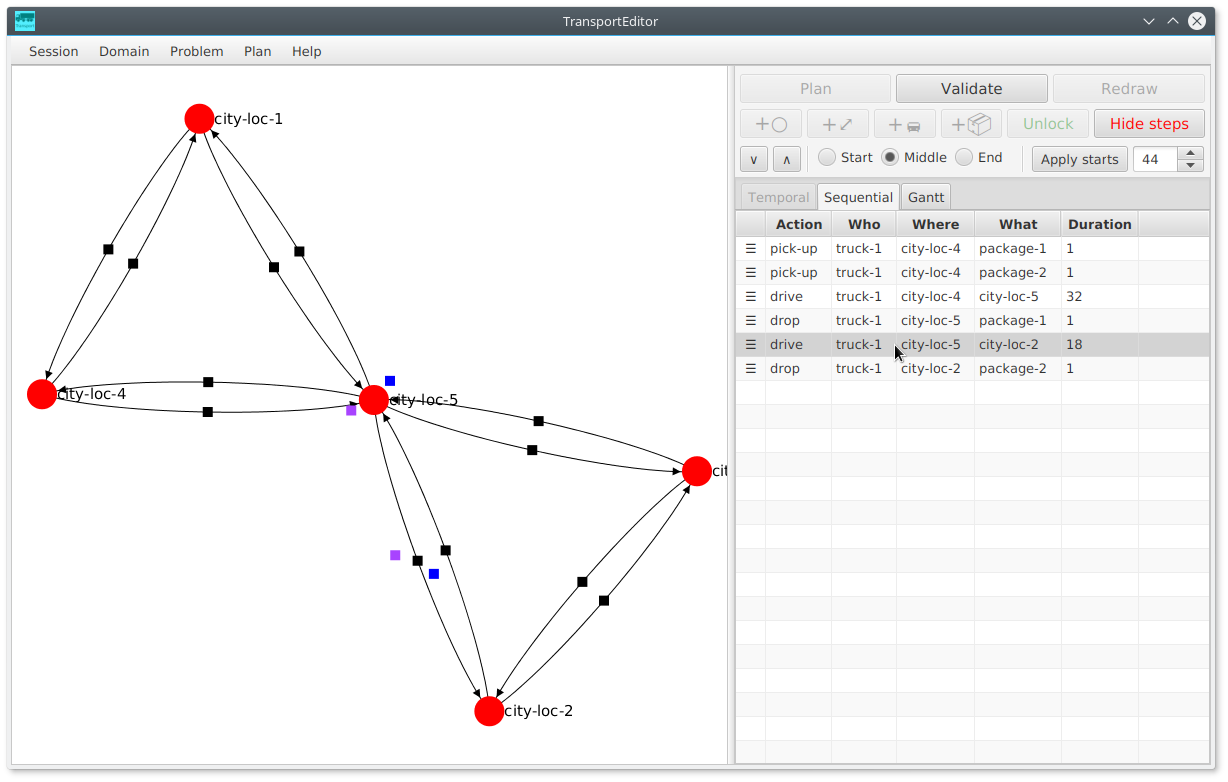
\includegraphics[width=1.0\textwidth]{../img/transporteditor_screenshot}
\end{center}
\caption{TransportEditor stepping through a plan of a simple sequential problem.}
\label{fig:transporteditor-screenshot}
\end{figure}

The basic workflow of TransportEditor consists of the following user's steps:
\begin{itemize}
\item Select which formulation of the Transport domain they want to work with or create their own variant.
\item Load the PDDL or create their own problem of the given domain.
\item TransportEditor draws the given graph as good as it can.
\item Iterate among the following options:
\begin{itemize}
\item Load a planner executable and let TransportEditor run the planner on the loaded problem instance for a given time, then load the resulting plan.
\item Load a pre-generated plan.
\item Step through the individual plan actions and let TransportEditor visualize them.
The user can go forward and backward in the plan and inspect each step in great detail.
\item Edit the graph: add/remove/edit the location or properties of vehicles, packages, roads, locations and possibly petrol stations.
\item Save the currently generated plan.
\item Save the problem (along with the graph drawing hints).
\item Save the domain (export to a PDDL file).
\end{itemize}
\item Save and close the currently loaded problem. Exit the application or go back to the first step.
\end{itemize}

TransportEditor is a part of this thesis and you can find it on the attachment CD (see the attached \nameref{cd-contents} for more information). Both the \nameref{transporteditor-user-manual} and
the \nameref{transporteditor-developer-documentation} are attached to this thesis, along with the \nameref{transporteditor-developer-javadoc} in a digital form.

\TODO{Expand this section with \citep{Skopek2017}}

\chapter{Transport domain problem analysis}

\section{Problem instances}

\TODO{Datasets}

\section{Problem features}

\section{TransportEditor -- a Transport domain planning environment}

TransportEditor aims to be a problem editor and plan visualizer for the Transport domain.
It is an intuitive GUI desktop application for making quick changes and re-planning, but also designing a new problem dataset from scratch. TransportEditor will help researchers working on this domain fine-tune their planners; they can visualize the various corner cases their planner fails to handle, step through the generated plan and find the points where their approach fails.
A secondary motivation is to be able to test approaches for creating plans for the domain.

The basic workflow of TransportEditor consists of the following user's steps:
\begin{itemize}
\item Select which formulation of the Transport domain they want to work with or create their own variant.
\item Load or create their own problem of the given domain. See section \ref{input-output} for details on the input format.
\item TransportEditor draws the given graph as good as it can.
\item Iterate among the following options:
\begin{itemize}
\item Load a planner executable and let TransportEditor run the planner on the loaded problem instance for a given time, then load the resulting plan.
\item Load a pre-generated plan.
\item Step through the individual plan actions and let TransportEditor visualize them.
The user can go forward and backward in the plan and inspect each step in great detail.
\item Edit the graph: add/remove/edit the location or properties of vehicles, packages, roads, locations and possibly petrol stations.
\item Save the currently generated plan.
\item Save the problem (along with the graph drawing hints).
\item Save the domain (export to a PDDL file).
\end{itemize}
\item Save and close the currently loaded problem. Exit the application or go back to the first step.
\end{itemize}

TransportEditor is a part of this thesis and you can find it on the attachment DVD, in the folder \TODO{releases}. If you want to find out more details about it, see the attached TransportEditor User Manual\ref{transporteditor-user-manual},
the TransportEditor Developer Documentation\ref{transporteditor-developer-documentation}
and the TransportEditor Developer JavaDoc\ref{transporteditor-developer-javadoc}.




\chapter{Planning Transport domain problems}

\section{Planner overview}

\section{Domain independent planners}

\subsection{FastDownward}

\section{Simple Greedy BFS}

\section{Forward planning}

\subsection{Heuristic}

\section{OptaPlanner}

\TODO{Formulate as CSP?}

\section{Neural combinatorial optimization}

\TODO{Leave this out?}

\section{Planner result comparison}

\TODO{compare to original conference results too}


\chapter*{Conclusion}
\addcontentsline{toc}{chapter}{Conclusion}

\TODO{conclusion}

\section*{Future work}
\addcontentsline{toc}{section}{Future work}

\TODO{Mention future work}


%%% Bibliography
%%% Bibliography (literature used as a source)
%%%
%%% We employ bibTeX to construct the bibliography. It processes
%%% citations in the text (e.g., the \cite{...} macro) and looks up
%%% relevant entries in the bibliography.bib file.
%%%
%%% The \bibliographystyle command selects, which style will be used
%%% for references from the text. The argument in curly brackets is
%%% the name of the corresponding style file (*.bst). Both styles
%%% mentioned in this template are included in LaTeX distributions.

%\bibliographystyle{plainnat}    %% Author (year)
\bibliographystyle{unsrt}     %% [number]

\renewcommand{\bibname}{Bibliography}

%%% Generate the bibliography. Beware that if you cited no works,
%%% the empty list will be omitted completely.

\bibliography{bibliography}

%%% If case you prefer to write the bibliography manually (without bibTeX),
%%% you can use the following. Please follow the ISO 690 standard and
%%% citation conventions of your field of research.

% \begin{thebibliography}{99}
%
% \bibitem{lamport94}
%   {\sc Lamport,} Leslie.
%   \emph{\LaTeX: A Document Preparation System}.
%   2nd edition.
%   Massachusetts: Addison Wesley, 1994.
%   ISBN 0-201-52983-1.
%
% \end{thebibliography}


%%% Figures used in the thesis (consider if this is needed)
\listoffigures

%%% Tables used in the thesis (consider if this is needed)
%%% In mathematical theses, it could be better to move the list of tables to the beginning of the thesis.
\listoftables

%%% Abbreviations used in the thesis, if any, including their explanation
%%% In mathematical theses, it could be better to move the list of abbreviations to the beginning of the thesis.
\chapwithtoc{List of Abbreviations}

AI --- Artificial Intelligence\\
API --- Application Programming Interface\\
BFS --- Breadth-First Search\\
CSP --- Constraint Satisfaction Problem\\
CVRP --- Capacitated Vehicle Routing Problem\\
DFS --- Depth-First Search\\
HC --- Hamiltonian Circuit (Cycle)\\
HTN --- Hierarchical Task Network\\
ICAPS --- International Conference on Automated Planning and Scheduling\\
IPC --- International Planning Competition\\
MDVRP --- Multiple Depot Vehicle Routing Problem\\
PDDL --- Planning Domain Definition Language\\
SFA* --- Sequential Forward A*\\
STRIPS --- Stanford Research Institute Problem Solver\\
TSP --- Traveling Salesman Problem\\
tqe --- Temporally Qualified Expression\\
VRP --- Vehicle Routing Problem\\

%%% Attachments to the bachelor thesis, if any. Each attachment must be
%%% referred to at least once from the text of the thesis. Attachments
%%% are numbered.
%%%
%%% The printed version should preferably contain attachments, which can be
%%% read (additional tables and charts, supplementary text, examples of
%%% program output, etc.). The electronic version is more suited for attachments
%%% which will likely be used in an electronic form rather than read (program
%%% source code, data files, interactive charts, etc.). Electronic attachments
%%% should be uploaded to SIS and optionally also included in the thesis on a~CD/DVD.
%%% Allowed file formats are specified in provision of the rector no. 23/2016.
\chapwithtoc{Attachments}

\section*{TransportEditor User Manual}

%%%% manual_en

%%%% END manual_en


\section*{TransportEditor Developer Documentation}

%%%%%%%%% README
TransportEditor aims to be a problem editor and plan visualizer for the Transport domain from the IPC 2008.
The goal is to create an intuitive GUI desktop application for making quick changes and re-planning,
but also designing a new problem dataset from scratch.

\subsection*{Getting help}

\textbf{For users looking for help}: a manual describing all possible features of TransportEditor is available in the app itself:
in the upper menu bar item \textbf{Help $\to$ Help}.

Post any development questions or comments you may have on Stack Overflow and/or don't hesitate to
\href{https://gitlab.com/oskopek/TransportEditor/issues}{open an issue}.

\subsection*{Running TransportEditor releases}
\begin{itemize}
\item Download a release from:\\ \url{https://github.com/oskopek/TransportEditor/releases}

\item Note: TransportEditor uses \href{http://semver.org/}{semantic versioning}.

\item To directly run TransportEditor, download the \textbf{executable JAR file}: \texttt{TransportEditor-VERSION-jar-with-dependencies.jar}

\item If you want to run a release, just try:\\ \texttt{java -jar TransportEditor-VERSION-jar-with-dependencies.jar}
\end{itemize}

\subsection*{Building \& running TransportEditor}\label{readme-building}

\begin{itemize}
\item See the section (further down) on How-to setup your \textbf{build environment} first.

\item \textbf{Recommended}: \texttt{mvn clean install -DskipTests}

\item To run \textbf{unit tests}: \texttt{mvn clean install}

\item To run \textbf{integration tests}: \texttt{mvn clean install -Pit}

\item To \textbf{clean}, run: \texttt{mvn clean}

\item To build \textbf{docs} too: \texttt{mvn clean install -Pdocs}

\item \textbf{Run TransportEditor}:
\begin{itemize}
\item If you followed the build environment setup and you want to run your version of TransportEditor,
run the command \texttt{mvn exec:java} from the \texttt{transporteditor-editor} module directory.

\item If you want to run a translated version of TransportEditor, set your system locale accordingly and restart TransportEditor. If you want to try out a translated version (on Linux), try:\\ \verb+LC_ALL="LOCALE" java -jar TransportEditor.jar+\\
Substitute \texttt{LOCALE} for any locale available on your system. To view all available locales,
run \verb+locale -a+.
\end{itemize}
\end{itemize}


\subsection*{Setup your build environment}
\begin{enumerate}

\item \textbf{Install Git}

\begin{itemize}

\item Fedora: \texttt{sudo dnf install git}

\item Ubuntu: \texttt{sudo apt-get install git}

\item Windows: Download and install Git for Windows at:\\ \url{https://git-scm.com/downloads}

\end{itemize}

\item \textbf{Install git-lfs} from \href{https://git-lfs.github.com/}{https://git-lfs.github.com/}

\item \textbf{Install Java8 JDK} -- \href{http://www.oracle.com/technetwork/java/javase/downloads/index.html}{Oracle JDK Downloads} -- Select: Java Platform (JDK)

\begin{itemize}

\item \textbf{NOTE}: You need \texttt{jdk-8u40} or newer (JavaFX 8 dependency).

\end{itemize}

\item \textbf{Install Maven} -- preferably the latest version you can.
Usually, your distribution's package management repository is enough:

\begin{itemize}

\item Fedora: \texttt{sudo dnf install mvn}

\item Ubuntu: \texttt{sudo apt-get install maven}

\item Windows: See: \href{http://maven.apache.org/guides/getting-started/windows-prerequisites.html}{Maven on Windows}
 and \href{http://maven.apache.org/download.cgi}{Maven Downloads}.

\end{itemize}

\item \textbf{Fork the repository} -- Create a fork of the \href{https://gitlab.com/oskopek/TransportEditor/}{oskopek/TransportEditor repository}
(under the logo) on GitLab, usually the fork will be called: \texttt{yourusername/TransportEditor}.

\item \textbf{Clone the your fork} -- run:\\ \texttt{git clone \href{https://gitlab.com/yourusername/TransportEditor.git}{https://gitlab.com/yourusername/TransportEditor.git}}\\
Or, preferably, use SSH:\\ \texttt{git clone \href{mailto:git@gitlab.com}{git@gitlab.com}:yourusername/TransportEditor.git}

\item \textbf{Pull the LFS files} -- run: \texttt{git lfs pull}

\item \textbf{Run the build} (see: \nameref{readme-building})
\end{enumerate}

\subsection*{Short design description}
The model for the Transport domain is pretty complicated,
because it handles:

\begin{itemize}
\item Multiple variants of the Transport domain

\item Planning and visualization with the same model
\end{itemize}

That's what this short section is for -- describing the ideas behind the model, so that reading the code
afterwards is easier. The model is split into 4 parts:

\begin{itemize}
\item Session
\item Domain
\item Problem
\item Plan
\end{itemize}

\subsection*{Plan}
The plan consists of an ordered list of actions.
There are two types of plans:

\begin{itemize}
\item Sequential -- these plans are strictly linear, actions do not overlap (imagine simple linked list).
\item Temporal -- every action in this plan has a time interval in which it takes place.
This plan is basically a set of intervals with associated actions. For storing it, we use an
\href{https://en.wikipedia.org/wiki/Interval_tree}{Interval tree},
which allows efficient access to actions given a time or time range.
\end{itemize}

\subsubsection*{Visualizing plans}

There are currently two ways to visualize both plan types:

\begin{itemize}
\item Simple list -- both sequential and temporal versions look similar. Both are filterable by right clicking on the headers.
\begin{itemize}
\item Sequential: uses a simple drag-and-drop reorderable table of action arguments.
See the screenshot on the top of the README for a preview. Is redrawn completely after every change.

\item Temporal: in contrast to the sequential variant, this one cannot be reordered by dragging. The start times can however
be edited, which will result in the table reordering itself. Is not redrawn completely, adjusts its internal state and
redraws the necessary parts.
\end{itemize}

\item Gantt chart -- both sequential and temporal versions look alike, resembling a XY chart, the X axis being the time
axis and the Y axis having all action objects. Both are redrawn every time the plan changes or it's filter
in the simple list is changed.
\begin{itemize}
\item Sequential: using it to visualize sequential plans is not very interesting, as it offers almost no added insights on top of the simple list

\item Temporal: when visualizing temporal plans with a Gantt, we can observe the synchronicity of planned actions
and, to some extent, the cooperation of individual actors
\end{itemize}
\end{itemize}

\subsubsection*{Persisting plans}
Using string manipulation and built-in constants and format, it is persisted into a VAL-like format.
For parsing, we assume a correct and valid VAL-like plan. A very simple string manipulation and Regex-based approach
is used for both temporal and sequential plans. Additionally, a simple \href{http://www.antlr.org/}{ANTLR} grammar
is used in some places. See the \texttt{persistence} package for details.

\subsection*{Problem}
The problem is basically a graph (with multiple possible ``layers'', f.e. fuel) and a vehicle and package map.

Currently we use \href{http://graphstream-project.org/}{GraphStream} for both the data storage and visualization of the graph.
Apart from nodes and edge arrows, everything else is visualized as
``\href{http://graphstream-project.org/doc/Tutorials/Graph-Visualisation/#sprites}{sprites}''.


Fuel is added as different graph edge type (\verb+FuelRoad+ instead of \verb+DefaultRoad+) and a domain label change
(see \verb+PddlLabel+s in the domain).
If the domain is fuel enabled, the fuel properties of locations, roads and vehicles else will be displayed.


\subsubsection*{Visualizing problems}

Problem visualization does not fundamentally differ between different domains and problems.
Some problem tooltips/properties might dis/appear when changing the domain type.


The graph is automatically laid out using a \texttt{SpringBox} algorithm from GraphStream
for a given time and then switched to manual layout.

\subsubsection*{Persisting problems}
Both rule pages of \href{http://icaps-conference.org/ipc2008/deterministic/CompetitionRules.html}{IPC-6}
and \href{https://helios.hud.ac.uk/scommv/IPC-14/rules.html}{IPC-8}
specify PDDL 3.1 as their official modelling language (language for domain
and problem specification).
Daniel L. Kovacs proposed an updated and corrected BNF (Backus-Naur Form)
\href{https://helios.hud.ac.uk/scommv/IPC-14/repository/kovacs-pddl-3.1-2011.pdf}{definition of PDDL 3.1}.


Using a \href{http://freemarker.org/}{Freemarker} template and a lot of string manipulation it is persisted into PDDL.
For parsing, we assume a correct and valid problem and use a formal grammar written in \href{http://www.antlr.org/}{ANTLR}
to parse PDDL into a generated code structure provided by ANTLR and the \texttt{maven-antlr-plugin}. The same grammar as for
domains is used. See the \texttt{persistence} package and the \texttt{src/main/antlr4} folder for details.


\subsection*{Domain}
There is basically only one domain type: \texttt{VariableDomain} (we also have the notion of a \texttt{SequentialDomain},
but it is basically just an in-code hardcoded equivalent of loading the sequential Transport domain PDDL
into a \texttt{VariableDomain}).


The domain contains flags (labels), telling us which ``layers'' are enabled and which are not.
The UI, validator, IO and planner all take these into account.
It also contains methods for action creation using their correct domain-specified definitions
and provides other useful data (predicates, functions, \ldots).


\subsubsection*{Visualizing domains}

Domains are not visualizable per se.

\subsubsection*{Persisting domains}
Using a \href{http://freemarker.org/}{Freemarker} template and a lot of string manipulation it is persisted into PDDL.
For parsing, we assume a correct and valid problem and use a formal grammar written in \href{http://www.antlr.org/}{ANTLR}
to parse PDDL into a generated code structure provided by ANTLR and the \texttt{maven-antlr-plugin}. The same grammar as for
problems is used.

TransportEditor doesn't load the PDDL domain definitions directly -- those are already built-in.
We only read the domain files to check which subset of conditions the user has chosen to model.

In the UI, we can also create a domain using a popup dialog backed by a \texttt{VariableDomainBuilder} in the background.
It is essentially switchboard for gathering the appropriate flags and other properties the domain should have.

\subsection*{Session}
The session is where everything comes together. It keeps an instance of the domain, problem and plan (and planner and
validator, \ldots). We can use it to reason about what actions can be executed in the UI with the currently loaded
objects and also as a quick persistence solution -- if you save a session, you can then load it next time and
do not have to open all the individual parts again.


\subsubsection*{Visualizing sessions}

Sessions are visualized by visualizing all their (possible) parts.

\subsubsection*{Persisting sessions}
Sessions are persisted automatically to XML using \href{https://x-stream.github.io/}{XStream}. This means, all its properties
should be reasonably serializable (by reflection).

\subsection*{Planning}
Any class implementing the \texttt{Planner} interface can be set as the planner for a session and if it has all the properties
that are needed (domain \& problem), we can generate a plan using an instance of that class. TransportEditor supports
external (executable) planners out of the box, given that the executable adhere to a few rules (for details, see
\texttt{ExternalPlanner}). An end of planning event is raised after planning finishes, for UI redrawing purposes.

\subsection*{Validation}
Any class implementing the \texttt{Validator} interface can be used as a validator for plans in a planning session.
Validation happens automatically after planning in a session or it can be triggered manually. There are different
validators with different strictness (used for different domain variants). Choosing a wrong combination of domain,
problem and validator might cause false positives or false negatives, make sure to read the documentation of the
individual validators. TransportEditor supports a popular external validator called VAL, out of the box.

\subsection*{General notes}
There are few other small features of the project worth mentioning.

\subsubsection*{CDI \& the EventBus}
CDI (Context and Dependency Injection) using \href{http://weld.cdi-spec.org/}{Weld} is used for inversion of control
and for communication without tight coupling. Should only be used in the UI part of the project.


For event-driven communication on the front end, Guava's \texttt{EventBus} is used. Again, it enables persistent
reactive handling without tight coupling.

\subsubsection*{JavaFX properties and bindings}
The JavaFX based UI makes heavy use of bindings and properties, essential features of JavaFX. They enable
reactive changes to the UI in an efficient manner, but can be a bit tricky when reading code that uses them.
For even more power, we use the \href{http://fxexperience.com/controlsfx/}{ControlsFX} library, but try to avoid it,
if possible.

\subsubsection*{Model immutability}
The model (mainly the package \texttt{com.oskopek.transporteditor.model}) is designed to be immutable
(excluding a few exceptions). This makes it easier to reason about complex, possibly multithreaded operations
on top of it. This note is useful to keep in mind when reading code that changes the model data.

\subsubsection*{Tests}
The project aims to be well tested and verified. To stick to these goals, we have several levels of tests,
that are run by a CI (Continuous Integration) system after every push and should also be run by developers
(at least) after every commit. The displayed test coverage in the README is calculated as an average of unit
and integration test coverage.


TransportEditor currently has 3 types of tests:

\begin{itemize}
\item Unit tests (\texttt{*Test.java}) -- simple and quick to run tests that test one thing and test it well.

\item Integration tests (\texttt{*IT.java}) -- complex tests that handle multiple moving parts at once. Usually involving IO or
other not easily mockable things. Try to avoid abusively writing these in favour of unit tests, if possible.

\item User interface tests (\texttt{*UI.java}) -- test the UI using \href{https://github.com/TestFX/TestFX}{TestFX}.
At the moment, they are under-represented and not run very often. Currently, CI doesn't run them by default.
\end{itemize}


\subsubsection*{Comments, code style}
TransportEditor employs a rigorous code style checker called \texttt{checkstyle} that is run automatically at every build.
Please adhere to that style when extending/editing the code base. Multiple other unwritten and unspecified rules might
apply. Please, do not take any style comments personally -- they are in place so that the code remains in tact and
readable in the long term.

As part of the \texttt{checkstyle} process, JavaDoc comments are enforced on every method and class (excluding tests).
They should briefly describe the design/implementation choices, \textbf{why} they were made and any useful examples and or
other quirks.
%%%%%%%%% ENDREADME



\openright
\end{document}
